% !TEX program = pdflatex
\documentclass[11pt,a4paper]{article}

\usepackage[T1]{fontenc}
\usepackage[utf8]{inputenc}
\usepackage{lmodern}
\usepackage{microtype}
\usepackage[margin=1in]{geometry}
\usepackage{booktabs}
\usepackage{tabularx}
\usepackage{enumitem}
\usepackage{xcolor}
\usepackage{tikz}
\usetikzlibrary{arrows.meta,positioning,fit,shapes.geometric,calc}
\usepackage[hidelinks,colorlinks=true,linkcolor=blue!50!black,citecolor=blue!50!black,urlcolor=blue!50!black]{hyperref}
\usepackage{framed}

\sloppy

% ---- side boxes -------------------------------------------------------------
\definecolor{boxbg}{rgb}{0.96,0.97,0.99}
\definecolor{boxrule}{rgb}{0.30,0.40,0.55}
\newenvironment{aside}[1][Aside]{%
  \def\FrameCommand{\fboxsep=8pt\fcolorbox{boxrule}{boxbg}}%
  \MakeFramed{\advance\hsize-2\fboxsep\FrameRestore}%
  \noindent\textbf{#1.}\par\smallskip%
}{\endMakeFramed}

\definecolor{warnbg}{rgb}{0.99,0.96,0.92}
\definecolor{warnrule}{rgb}{0.65,0.40,0.10}
\newenvironment{warning}[1][Watch out]{%
  \def\FrameCommand{\fboxsep=8pt\fcolorbox{warnrule}{warnbg}}%
  \MakeFramed{\advance\hsize-2\fboxsep\FrameRestore}%
  \noindent\textbf{#1.}\par\smallskip%
}{\endMakeFramed}

\setlength{\parskip}{0.4em}
\setlength{\parindent}{0pt}

\title{\textbf{E-Ring Voting --- Explain Like I'm Five}\\[0.4em]
       \large A walk-through with no math, for a curious high-schooler}
\author{Daniele Lin \and Niccol\`o Pagano}
\date{May 2026}

\begin{document}
\maketitle

\begin{quote}
\itshape
This document explains a small computer-science research project we
built. It is written for a smart high-school student who has done a bit
of programming and is curious about how online voting could actually
work. There are no equations in this document --- just analogies, a
few diagrams, and a careful build-up of the ideas. If you want the
mathematical version, the file \texttt{notes.tex} in the same folder
covers the same material as a university-level walk-through.

By the end of this you should be able to explain to a friend
\emph{what the project does}, \emph{why it is harder than it sounds},
and \emph{what we think we got right and wrong}.
\end{quote}

\tableofcontents

% ===========================================================================
\section{What's the point?}
% ===========================================================================

We built a small system for running \textbf{anonymous online votes}
that also lets anyone in the world \textbf{check the result}. Think of
a class president election, a board vote in a company, or a small
referendum --- not a national election.

Two properties have to be true at the same time:

\begin{itemize}[leftmargin=*]
  \item \textbf{Nobody can tell how you voted.} Not the people running
        the election, not the developers, not anyone who reads the
        public record of the vote.
  \item \textbf{Anyone can recompute the result.} Given the public
        record of the election, you can do the count yourself, with
        your own laptop, and refuse to accept any other claimed result.
\end{itemize}

If you stop and think about it for a minute, those two properties look
like they contradict each other. ``The votes are secret'' usually
means ``trust us, you can't see them.'' ``Anyone can recompute''
usually means ``the votes are public.'' How can both be true?

The whole project is built around one mathematical trick that breaks
the contradiction. The rest of these notes explain the trick (in
words), what we built around it, and where the limits are.

% ===========================================================================
\section{The contradiction, in concrete terms}
% ===========================================================================

Imagine your class is voting on lunch. The options are pasta, pizza,
\textit{focaccia}. You write your choice on a slip of paper and drop
it in a sealed box. At the end of the period, the teacher opens the
box and counts.

What can go wrong?

\begin{itemize}[leftmargin=*]
  \item \textbf{The teacher cheats on the count.} You can't tell, because
        you're not the one counting. Maybe the teacher swaps two
        ballots, or pretends one didn't exist.
  \item \textbf{The teacher peeks at who voted for what.} You can't tell,
        because they own the box.
  \item \textbf{Someone votes twice.} The teacher might or might not
        notice; you certainly can't.
\end{itemize}

\textbf{The naive online version is worse.} The website stores your
vote in a database. The database administrator can read it. The server
can lie about the count. You have to trust a stranger to be honest, and
even if they are honest, you have to trust they wrote the code right.

What we want is a system where:

\begin{enumerate}[leftmargin=*]
  \item Your ballot, the very moment you cast it, is mixed in with
        everyone else's so well that even the people running the
        election can't tell which one is yours.
  \item Every ballot is written down in a public place that anyone
        can read.
  \item The rules of the system make it \emph{impossible} for a
        cheater to publish a fake count without it being publicly
        obvious.
\end{enumerate}

Property~1 sounds the most magical. Property~2 sounds easy. Property~3
sounds nice but vague. The next sections build up each one.

% ===========================================================================
\section{The magic envelope: ring signatures}
% ===========================================================================

Here is the key idea, in an analogy.

\begin{aside}[The crowd analogy]
Suppose 50 people are in a room. One of them stands up and shouts
\emph{``I am one of the 50 people in this room.''} You believe them
--- they can prove it by, say, holding up a list of all 50 names
including their own. But there is no way to tell \emph{which} of the
50 it was. They could be any of them.

A \textbf{ring signature} is the digital version of that. It is a way
to sign a message such that the signature proves \emph{``one of these
50 people signed this,''} without revealing which one.
\end{aside}

A real-world example you have probably encountered without realising:
when a whistleblower leaks something to a journalist and the journalist
says ``a source inside the company,'' the source is anonymous within
the crowd ``employees of the company.'' If the company has 5000
employees, the crowd is big enough to hide in. If the company has 3
employees, it isn't.

So if every voter in our election has a digital ``signature key'' (a
secret number only they know), and every voter publishes their
``signature lock'' (a public number that proves who they are), then we
can build the ballot like this:

\begin{itemize}[leftmargin=*]
  \item Alice wants to vote for pasta.
  \item She uses her secret key to produce a \emph{ring signature} on
        the word ``pasta.'' The ring is \emph{everyone's public
        locks}, including hers, mixed together.
  \item Anyone in the world can check the signature: it is valid, so
        \emph{one of the 50 registered voters} voted for pasta.
  \item Nobody can tell it was Alice. Not even the teacher.
\end{itemize}

This is property 1 from before. The ballot is publicly visible, but
the \emph{voter} is hidden inside the crowd of registered voters.

\begin{aside}[Why this is mathematically possible]
The math behind ring signatures uses something called \emph{public-key
cryptography} --- the same family of math that protects your bank
website (the little padlock in the browser). The trick is that with the
right kind of math, you can build a signature that depends on
\emph{at least one} person's secret key, but doesn't reveal
\emph{which} one. From the outside, all 50 possible signers look
equally likely to have produced it.

The exact construction we use was proposed in 2021 by two researchers,
Alessandra Scafuro and Bihan Zhang. The repository implements their
recipe step by step.
\end{aside}

% ===========================================================================
\section{The double-vote problem}
% ===========================================================================

If the ballot hides the voter, what stops Alice from voting twice?

Plain ring signatures don't stop her. She could sign ``pasta'' once,
then sign ``pizza'' again, and there would be no way to tell that
both signatures came from the same person.

The fix is a feature called \textbf{one-time traceability}, which is
what the ``T'' in our project name (e-\textbf{R}ing-voting + one-time
\textbf{T}raceable) refers to. Here is the analogy:

\begin{aside}[The wax-seal analogy]
Imagine that when you sign a ballot, the signature automatically
imprints a unique seal --- like a wax stamp --- that depends only on
\emph{you} and \emph{this election}. The seal is the same every time
\emph{you} sign in \emph{this} election, no matter what the ballot
says. But the seal is also \emph{cryptographically scrambled} so that
nobody can read it as ``this is Alice's seal'' --- it just looks like
random noise.

\medskip
Now consider what happens if Alice signs two different ballots
(``pasta'' and ``pizza''):
\begin{itemize}
  \item The two signatures have the same scrambled seal --- because
        both came from Alice in this election.
  \item Anyone comparing the two ballots can see ``hey, these have a
        matching seal --- the same person produced both.''
  \item And, by a bit of further math, the matching seal actually
        reveals \emph{which} voter (which public lock) it belongs to.
        So Alice is publicly named as the cheater.
\end{itemize}

\medskip
But if Alice signs only \emph{once}, her seal is on exactly one
ballot. No other ballot has it. So the seal stays scrambled,
unreadable, and Alice remains anonymous inside the 50-voter ring.
\end{aside}

This is the cleverest part of the whole system. The same signature
both \emph{protects} you when you behave honestly and
\emph{exposes you} the moment you try to cheat.

\begin{warning}
This trick works \emph{only within one election}. A different
election has a different seal-recipe, so Alice's seal looks completely
different from one election to the next. You cannot use it to track a
voter across elections.
\end{warning}

% ===========================================================================
\section{Where do you write everything down?}
% ===========================================================================

Anonymity (the ring signature) and one-vote-per-person (the traceable
seal) are the cryptographic core. But for an auditor to actually
\emph{check the count}, the ballots have to live somewhere public.

We call this public place the \textbf{bulletin board}. Think of it as
a notice board in the middle of a town square. Anyone can read it.
Nobody can erase entries. Every new entry shows the time it was
posted. And every entry has a tiny pointer to the previous entry, so
you can scroll back through the entire history.

\begin{center}
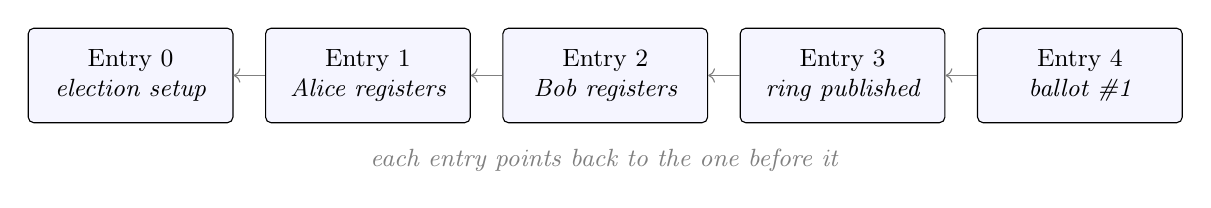
\begin{tikzpicture}[
  every node/.style={font=\small},
  entry/.style={draw, rounded corners=2pt, minimum width=2.6cm, minimum height=1.2cm, fill=blue!4},
]
\node[entry] (e0) {\shortstack{Entry 0\\\itshape election setup}};
\node[entry, right=0.4cm of e0] (e1) {\shortstack{Entry 1\\\itshape Alice registers}};
\node[entry, right=0.4cm of e1] (e2) {\shortstack{Entry 2\\\itshape Bob registers}};
\node[entry, right=0.4cm of e2] (e3) {\shortstack{Entry 3\\\itshape ring published}};
\node[entry, right=0.4cm of e3] (e4) {\shortstack{Entry 4\\\itshape ballot \#1}};
\draw[->, gray] (e1) -- (e0);
\draw[->, gray] (e2) -- (e1);
\draw[->, gray] (e3) -- (e2);
\draw[->, gray] (e4) -- (e3);
\node[below=0.2cm of e2, gray] {\textit{each entry points back to the one before it}};
\end{tikzpicture}
\end{center}

The key property: \textbf{if anyone tries to silently edit an old
entry, the pointer chain breaks.} The whole point of the chain is to
make tampering loud --- a single changed byte invalidates every entry
that came after.

\textbf{The state of the election goes through phases on the board:}

\begin{enumerate}[leftmargin=*]
  \item \textbf{Setup.} The election parameters are written: options
        (pasta / pizza / focaccia), the schedule (when voting opens
        and closes), and who is allowed to run the election.
  \item \textbf{Registration.} Each voter's public lock is added.
        After registration closes, the list of voters is frozen.
  \item \textbf{Ring.} The frozen list is published as ``the ring'' ---
        the official anonymity crowd. From now on, ring signatures
        from anyone in this crowd are valid ballots.
  \item \textbf{Ballots.} Voters cast their ring-signed ballots. Each
        one gets a new line on the bulletin board.
  \item \textbf{Closed.} When the schedule says voting is over, the
        bulletin board is sealed.
  \item \textbf{Tally.} The organisers publish their count --- but
        crucially, anyone can recompute it from the public ballots
        and contradict them if they cheat.
\end{enumerate}

% ===========================================================================
\section{Who is allowed to write on the board?}
\label{sec:who}
% ===========================================================================

This is where the project gets interesting, because there are two very
different sensible answers, and we implemented \emph{both} so we could
compare them.

\subsection{Option A: a small named team (the ``federated'' answer)}

A small group of named people --- say, 3 trusted scrutineers,
publicly identified by name --- jointly run the bulletin board. To
write a new entry, at least 2 of the 3 have to digitally co-sign it.

\begin{itemize}[leftmargin=*]
  \item \textbf{Good news:} fast. No expensive computation. Everyone
        knows who they are.
  \item \textbf{Good news:} a corrupt minority can't cheat. If
        scrutineer~1 alone tries to add a fake ballot, scrutineers~2
        and~3 refuse to sign and the entry is invalid.
  \item \textbf{What if two of them go bad together?} We add another
        layer: a separate group of \emph{witnesses} (say, three more
        named observers) who occasionally take a snapshot of the
        board and sign it. If the two corrupt scrutineers tried to
        show ``ledger version A'' to one witness and ``ledger version
        B'' to another, the two witnesses would later disagree on
        what they saw, and the disagreement is mathematical proof
        of cheating.
\end{itemize}

This is the same family of system as the one that secures HTTPS
certificates on the web (``Certificate Transparency''), and the same
shape as Sigsum (used for signed software releases). It is a
well-known pattern for keeping known parties honest.

\subsection{Option B: anybody can write (the ``blockchain'' answer)}

The other answer is the Bitcoin-style answer: don't pick a small named
team at all. Instead, \emph{anyone} on the internet can compete to
add the next entry. The competition is solving a small puzzle (the
``proof of work''): basically, your computer guesses random numbers
until one of them, when hashed, has enough leading zeros. The first
person to find a good number gets to add the next block of ballots,
and gets paid a small reward.

\begin{aside}[Why the puzzle?]
The puzzle exists to make it expensive to take over the system. If
adding entries were free, anyone could pretend to be a thousand
different identities at once and stuff the chain with fake entries.
The puzzle forces each ``identity'' to do real computational work,
which costs electricity, which costs money. So a faker has to pay for
every block they add.
\end{aside}

\begin{itemize}[leftmargin=*]
  \item \textbf{Good news:} no named team. Anyone with a computer can
        participate. No genesis-pinned trust.
  \item \textbf{Bad news:} the puzzle is slow (blocks take minutes,
        not seconds). The system runs an internal mini-currency
        (``eVotes'') to pay the puzzle-solvers.
  \item \textbf{Bigger bad news:} for an election that matters
        politically, an attacker can \emph{rent} a huge amount of
        computer power online (services like NiceHash sell hashrate
        by the hour). If their incentive --- e.g., swinging the
        outcome of a corporate-board election worth millions of
        dollars --- is bigger than what it costs to rent the
        computing power for the voting window, they win. This is the
        argument that Park and Specter (MIT, 2021) made in a famous
        paper called \textit{Going from bad to worse: from internet
        voting to blockchain voting.}
\end{itemize}

\subsection{The honest comparison}

\begin{center}\small
\begin{tabularx}{\linewidth}{l X X}
\toprule
& \textbf{Option A (named team)} & \textbf{Option B (open mining)} \\
\midrule
Who can write?           & A known team (e.g., 2-of-3 scrutineers) & Anyone with a computer \\
How fast?                & Seconds                                  & Minutes (slow on purpose) \\
Operating cost?          & Just the team's time                     & Electricity for the puzzle \\
Built-in currency?       & No                                        & Yes (otherwise nobody mines) \\
Best protection against? & A corrupt minority of the team           & A corrupt minority of miners \\
Weakest if?              & The team unanimously corrupts             & Someone rents enormous hashpower \\
\bottomrule
\end{tabularx}
\end{center}

\textbf{Neither is universally better.} The named-team option works
when the election has named accountable scrutineers (a school senate,
a co-op board, an inter-institution committee). The blockchain option
works when there is genuinely \emph{no} group anyone trusts to be the
team --- even a small one. The cost of that second case is that you
have to defend against rented-hashpower attacks, which gets
\emph{harder} the higher the political stakes.

% ===========================================================================
\section{What this project actually built}
% ===========================================================================

We built both options. The repository is split into three folders:

\begin{itemize}[leftmargin=*]
  \item \texttt{otrs/} --- the cryptography (the magic envelope + the
        seal trick). About 1{,}100 lines of Python. Used by both
        options below.
  \item \texttt{voting/} --- Option A, the named-team bulletin board.
        About 1{,}800 lines.
  \item \texttt{chain/} --- Option B, the proof-of-work chain. About
        1{,}400 lines.
\end{itemize}

Plus 127 automated tests that check the whole thing actually works
the way we say it does.

We also ran benchmarks to compare. At 50 voters, the named-team
option finishes a complete election in about 1.1 seconds and
produces a 324~KB public record. The blockchain option finishes the
same election in about 3.0 seconds and produces a 344~KB record ---
so it is roughly $1.6\times$ slower and uses about $6\%$ more storage,
mostly because the proof-of-work puzzle has to be solved for every
block.

\textbf{Both options produce the same answer to the question
``who won.''} The cryptography that makes the votes anonymous and
catchable-if-double-counted is exactly the same; what differs is who
gets to write on the public record.

% ===========================================================================
\section{What this project did \emph{not} fix}
% ===========================================================================

It's important to be honest about what we did not solve. These are
real, hard, open problems --- not ones a small project can knock out.

\begin{itemize}[leftmargin=*]

  \item \textbf{Coercion.} If someone threatens you and says ``vote
        for pasta or I'll fire you,'' you might want to prove to them
        that you obeyed. With our system, you actually \emph{can}
        prove it (by revealing your seal-recipe), so a coercer can
        force you to comply. Fixing this is called
        \emph{coercion resistance} and requires significantly more
        machinery (a 2005 paper called JCJ is the canonical
        starting point). It is one of the most active open problems
        in voting research.

  \item \textbf{Compromised computers.} If a virus on your laptop
        secretly signs whatever it wants, the cryptography can't
        help you --- the system can't tell the difference between
        ``Alice clicked pasta'' and ``Alice's malware clicked
        pasta.'' Real deployments need hardware (smart cards, HSMs)
        and that is a different engineering project.

  \item \textbf{Quantum computers.} The math we rely on can be
        broken by a sufficiently large quantum computer (the
        algorithm is called Shor's). Those computers don't exist
        yet at scale, but if they do, our system will need to be
        re-built on top of different mathematics
        (``post-quantum cryptography'').

  \item \textbf{Ring size.} Right now, an election with 1000 voters
        has 1000-person rings, and each ballot's signature is about
        $64$~kilobytes. That's fine for small elections; it's not
        fine for nation-scale ones. The fix is a class of
        \emph{logarithmic-size} ring signatures (Triptych,
        Groth--Kohlweiss-style), which we did not implement.

  \item \textbf{Truly proving the cryptography.} The math is correct
        in the paper that proposed it, but our specific Python
        implementation has not been independently audited or
        machine-checked using formal-verification tools like
        EasyCrypt. A machine-checked proof would be a research
        contribution in its own right.

\end{itemize}

% ===========================================================================
\section{How this connects to things you may have heard of}
% ===========================================================================

\paragraph{Bitcoin.} Bitcoin invented the proof-of-work chain we used
for Option~B. The difference is what is stored on the chain ---
Bitcoin stores money transfers, we store election records --- and
what we use it for. Most relevant to read first: Wikipedia on
``proof of work,'' then Nakamoto's 2008 Bitcoin whitepaper if you
want the original.

\paragraph{Certificate Transparency.} When your browser visits a
website, the website shows a certificate proving it owns the domain.
Certificate Transparency is a system of public bulletin boards that
record every certificate ever issued, so if a bad certificate
authority secretly issues a fake certificate for, say,
\texttt{gmail.com}, it gets logged publicly and the attack is
visible. Option~A in our project is the same idea, transplanted to
voting.

\paragraph{Voting research.} Two systems you might run into:
Helios (2008) is one of the earliest practical end-to-end-verifiable
voting systems. ElectionGuard (Microsoft, 2021) is more recent. Our
project sits in the same family but uses a different building block
(ring signatures) and is much smaller in scope.

% ===========================================================================
\section{Glossary}
% ===========================================================================

\begin{description}[leftmargin=1.2em, style=nextline, font=\bfseries]
  \item[Anonymity set] The crowd you are hiding inside. In our case,
        the set of registered voters in this election.
  \item[Ballot] A single voter's signed choice.
  \item[Bulletin board] The append-only public record where every
        election event is written. ``Append-only'' means new entries
        can be added but old entries cannot be edited or removed.
  \item[Election ID] A unique label for one specific election. The
        seal mentioned in the wax-seal analogy depends on it, which
        is why a voter's seal looks different in different elections.
  \item[Hash] A short fingerprint of a longer piece of data.
        ``SHA-256'' is the most common one. Changing even one bit of
        the input changes the fingerprint completely.
  \item[Mining] In Option~B, the activity of guessing nonces until
        the puzzle is solved. The reward for finding a good nonce is
        paid in eVotes.
  \item[Public-key cryptography] Math where you have a public ``lock''
        anyone can use to send you encrypted messages or verify your
        signatures, and a private ``key'' only you know that you use
        to read messages or produce signatures. The web's HTTPS
        padlock relies on this.
  \item[Ring signature] A signature that proves \emph{one of these
        $n$ people} signed it, without revealing which one.
  \item[Trace tag (``seal'' in this document)] The mathematical
        object that's the same every time a given voter signs in a
        given election. Collisions reveal a double-voter.
\end{description}

% ===========================================================================
\section*{What to read next}
% ===========================================================================

If you want the technical version of the same material, with the
actual mathematics, read \texttt{notes.tex} in this same folder
(25~pages). It walks through the same ideas with formulas, code
snippets, and a chapter on why the chain version is harder than it
looks.

If you want to skip the implementation details and read the
research-style write-up, read \texttt{paper/artifact.tex} (16~pages).
It is structured like a small academic paper.

If you want to read the code, the easiest starting point is
\texttt{otrs/otrs.py} --- the central file --- followed by
\texttt{tests/test\_otrs.py} which checks it works correctly.

\end{document}
